\documentclass[tikz,border=5pt]{standalone}
\usepackage[UTF8]{ctex}
\usepackage{amsmath,amssymb}
\usetikzlibrary{arrows.meta,calc}
\tikzset{>=Stealth,line cap=round,line join=round,
axis/.style={gray!70,thin},aux/.style={gray!65,dashed,thin},
incoming/.style={blue!75!black,very thick},
outgoing/.style={red!75!black,very thick},
optical/.style={green!45!black,thick}}
\begin{document}
% 1. Three actual parallel transverse planes in a common linear spatial projection.
\begin{tikzpicture}[font=\small,x={(.80cm,-.32cm)},y={(0cm,1.05cm)},z={(1.4cm,.34cm)}]
\foreach \zz/\label in {0/P_1,2.6/P_3,5.2/P_2}{
\fill[blue!4]plot[domain=0:360,samples=73]({cos(\x)},{sin(\x)},\zz)--cycle;
\draw[thick]plot[domain=0:360,samples=73]({cos(\x)},{sin(\x)},\zz);
}
\node[above left]at(-.9,1.35,0){$P_1$};
\node[above]at(0,1.25,2.6){$P_3$};
\node[above]at(0,1.25,5.2){$P_2$};
\draw[->,thick](0,0,-1.2)--(0,0,6.6)node[right]{$z$};
\draw[incoming,<->](-.88,0,0)--(.88,0,0);
\draw[outgoing,<->](0,-.88,5.2)--(0,.88,5.2);
\draw[optical,<->]({-.88*cos(35)},{-.88*sin(35)},2.6)
--({.88*cos(35)},{.88*sin(35)},2.6);
\draw[axis,->](0,0,0)--(1.5,0,0)node[right]{$x$};
\draw[axis,->](0,0,0)--(0,1.5,0)node[above]{$y$};
\draw[aux](0,0,2.6)--(1.05,0,2.6);
\draw[thin]plot[domain=0:35,samples=17]({.52*cos(\x)},{.52*sin(\x)},2.6);
\node at({.75*cos(17.5)},{.75*sin(17.5)},2.6){$\theta$};
\node[below]at(0,-.35,1.25){$I_1$};
\node[below]at(0,-.35,6.15){$I_2$};
\node at(0,-1.75,2.6){各元件的轴均位于横向 $x$--$y$ 平面};
\end{tikzpicture}
% 2. Actual projections for theta=30 degrees; amplitudes not intensities.
\begin{tikzpicture}[font=\small]
\begin{scope}
\draw[axis,->](0,-.3)--(0,2.5)node[above]{$y$};
\draw[axis,->](-.3,0)--(3.5,0)node[right]{$x$};
\draw[optical](-.45,-.2598)--(3.1,1.7898);
\draw[incoming,->](0,0)--(3,0)node[below]{$E_0$};
\draw[outgoing,->](0,0)--(2.25,1.299038);
\draw[aux](3,0)--(2.25,1.299038);
\fill(2.25,1.299038)circle(1.5pt);
\node[outgoing,above,rotate=30]at(1.3,.91){$E_0\cos\theta$};
\draw[thin](.7,0)arc(0:30:.7);
\node at(.95,.20){$\theta$};
\node[optical,above]at(3.1,1.79){$P_3$ 轴};
\node at(1.6,-.8){第一次：投影到 $P_3$};
\end{scope}
\begin{scope}[xshift=7cm]
\draw[axis,->](0,-.3)--(0,2.5)node[above]{$y$};
\draw[axis,->](-.3,0)--(3.5,0)node[right]{$x$};
\draw[optical](-.45,-.2598)--(3.1,1.7898);
\draw[outgoing,->](0,0)--(2.25,1.299038);
\draw[incoming,->](0,0)--(0,1.299038);
\draw[aux](2.25,1.299038)--(0,1.299038);
\fill(0,1.299038)circle(1.5pt);
\node[outgoing,above,rotate=30]at(1.8,1.38){$E_0\cos\theta$};
\node[incoming,left]at(-.2,.65){$E_0\cos\theta\sin\theta$};
\draw[thin](.606218,.35)arc(30:90:.7);
\node at(.47,.75){$\frac{\pi}{2}-\theta$};
\node at(1.6,-.8){第二次：投影到 $P_2$};
\end{scope}
\end{tikzpicture}
% 3. Signed local components add to the input exactly.
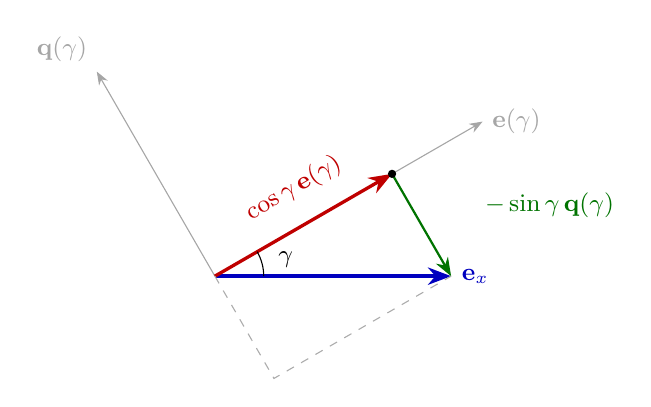
\begin{tikzpicture}[font=\small]
\draw[axis,->](0,0)--(3.4,1.96299)node[right]{$\mathbf e(\gamma)$};
\draw[axis,->](0,0)--(-1.5,2.598076)node[above left]{$\mathbf q(\gamma)$};
\draw[incoming,->](0,0)--(3,0)node[right]{$\mathbf e_x$};
\draw[outgoing,->](0,0)--(2.25,1.299038);
\draw[optical,->](2.25,1.299038)--(3,0);
\draw[aux](0,0)--(.75,-1.299038)--(3,0);
\fill(2.25,1.299038)circle(1.5pt);
\node[outgoing,above,rotate=30]at(1.15,.86){$\cos\gamma\,\mathbf e(\gamma)$};
\node[optical,right]at(3.3,.9){$-\sin\gamma\,\mathbf q(\gamma)$};
\draw[thin](.62,0)arc(0:30:.62);
\node at(.90,.21){$\gamma$};
\end{tikzpicture}
% 4. Reflection around the material axis; perpendicular components change sign.
\begin{tikzpicture}[font=\small]
\draw[aux](-.55,-.31754)--(3.3,1.90526);
\node[above right]at(3.3,1.90526){光轴 $\mathbf e(\gamma)$};
\draw[incoming,->](0,0)--(3,0)node[right]{$\mathbf e_x$};
\draw[outgoing,->](0,0)--(1.5,2.598076)node[above]{$\mathbf e(2\gamma)$};
\draw[thin](3,0)--(2.25,1.299038)--(1.5,2.598076);
\draw[optical,->](2.25,1.299038)--(1.82,2.04382);
\fill(2.25,1.299038)circle(1.6pt);
\draw[thin](.65,0)arc(0:30:.65);
\node at(.91,.20){$\gamma$};
\draw[thin](.866025,.5)arc(30:60:1);
\node at(.78,.83){$\gamma$};
\node[incoming,below]at(2.7,-.30){输入};
\node[outgoing,left]at(.68,1.62){输出};
\node at(1.4,-.95){沿光轴分量不变；正交分量相对反号};
\end{tikzpicture}
% 5. Time-parametric field loci, not arbitrary ellipse icons.
\begin{tikzpicture}[font=\small]
\foreach \yy in {0,-3.8}{
\foreach \xx in {0,5.3,10.6}{
\draw[axis](\xx-1.2,\yy)--(\xx+1.2,\yy);
\draw[axis](\xx,\yy-1.2)--(\xx,\yy+1.2);
}
\draw[incoming,thick](-1,\yy)--(1,\yy);
\draw[outgoing,thick](10.6-.5,\yy-.866025)--(10.6+.5,\yy+.866025);
}
\draw[optical,thick]plot[domain=0:360,samples=121]
({5.3+.75*cos(\x)-.25*sin(\x)},{.433012702*(cos(\x)+sin(\x))});
\draw[optical,thick](5.3,-3.8)circle(.707106781);
\foreach \yy/\a/\b in {0/30/30,-3.8/45/15}{
\draw[->,thick](1.45,\yy)--(3.80,\yy);
\draw[->,thick](6.75,\yy)--(9.1,\yy);
\node[above]at(2.6,\yy+.25){$Q_1:\ \beta_1=\a^\circ$};
\node[above]at(7.9,\yy+.25){$Q_2:\ \beta_2=\b^\circ$};
}
\node at(0,1.65){同轴叠加};
\node at(0,-2.1){圆偏振中间态};
\node at(0,-1.6){$x$ 向线偏振};
\node at(5.3,-1.6){椭圆偏振};
\node at(10.6,-1.6){$60^\circ$ 线偏振};
\node at(0,-5.4){$x$ 向线偏振};
\node at(5.3,-5.4){圆偏振};
\node at(10.6,-5.4){$60^\circ$ 线偏振};
\node at(5.3,-6.2){真实电场端点轨迹；各阶段总光强相同};
\end{tikzpicture}
% 6. The four full-transmission roots for theta2=60 degrees, in [0,180)^2.
\begin{tikzpicture}[font=\small]
\draw[->](0,0)--(7.85,0)node[right]{$\beta_1$};
\draw[->](0,0)--(0,7.85)node[above]{$\beta_2$};
\foreach \v in {45,90,135,180}{
\draw[axis](.04*\v,-.08)--(.04*\v,.08);
\draw[axis](-.08,.04*\v)--(.08,.04*\v);
\node[below]at(.04*\v,-.10){$\v^\circ$};
\node[left]at(-.1,.04*\v){$\v^\circ$};
\draw[gray!18](.04*\v,0)--(.04*\v,7.2);
\draw[gray!18](0,.04*\v)--(7.2,.04*\v);
}
\node[below left]at(-.1,-.1){$0$};
\fill[incoming](1.2,1.2)circle(2.5pt);
\fill[incoming](4.8,4.8)circle(2.5pt);
\fill[outgoing](1.8,.6)circle(2.5pt);
\fill[outgoing](5.4,4.2)circle(2.5pt);
\node[incoming,above right]at(1.2,1.6){$(30^\circ,30^\circ)$};
\node[incoming,above]at(4.8,5.05){$(120^\circ,120^\circ)$};
\node[outgoing,right]at(1.98,.50){$(45^\circ,15^\circ)$};
\node[outgoing,right]at(5.55,3.95){$(135^\circ,105^\circ)$};
\node at(3.6,7.80){目标轴：$\theta_2=60^\circ$};
\node[incoming]at(1.8,-.85){蓝点：同轴叠加};
\node[outgoing]at(5.5,-.85){红点：经圆偏振};
\end{tikzpicture}
\end{document}
